\documentclass[a4paper]{article}
\usepackage[warn]{mathtext}
\usepackage{graphicx} % Required for inserting images
\usepackage{wrapfig}
\usepackage{enumitem}
\usepackage[center]{caption}
\usepackage[english, russian]{babel}
\usepackage{amsmath}
\usepackage{geometry}
\setcounter{totalnumber}{5}

\geometry{verbose, a4paper, tmargin=2cm, bmargin=2cm, lmargin=2.0cm, rmargin=2.0cm}

\begin{document}
	
	\begin{titlepage}
		\centering
		{\scshape\Large МОСКОВСКИЙ ФИЗИКО-ТЕХНИЧЕСКИЙ ИНСТИТУТ \\
			(НАЦИОНАЛЬНЫЙ ИССЛЕДОВАТЕЛЬСКИЙ УНИВЕРСИТЕТ)\\ % название ВУЗа большим шрифтом
			Физтех-школа аэрокосмических технологий}
		
		\vspace{4cm} % отступ 4 см по вертикали
		{\LARGE Отчет о выполнении лабораторной работы 2.2.1}
		\vspace{1cm} % ещё 1 см
		
		{\huge\bf Исследование взаимной диффузии газов}
		
		\vspace{1cm} % ещё 1 см
		\vfill % заполнение по вертикали пустотой (LaTeX сам решит, сколько здесь отступить)
		
		\begin{flushright} % Этот текст будет с правого края страницы
			{\LARGE Губарев Никита, Б03-502}
		\end{flushright}
		\vfill 
		\today % Дата сборки документа
	\end{titlepage}
	\tableofcontents 
	\section{Аннотация}
	
	\section{Описание работы}
	\subsection{Теоретические сведения}
	
	Диффузией называют самопроизвольное взаимное проникновение веществ друг в друга, происходящее вследствие хаотичного теплового движения молекул. При перемешивании молекул разного сорта говорят о \textit{взаимной} (или концентрационной) диффузии.
	
	Диффузия в системе, состоящей из двух компонентов $a$ и $b$ (бинарная смесь), подчиняется закону Фика: плотности потока компонентов $j_{a,b}$ (количество частиц, пересекающих единичную площадку в единицу времени) пропорциональны градиентам их концентраций $\nabla n_{a,b}$, что в одномерном случае можно записать как
	\[
	j_a = -D \frac{\partial n_a}{\partial x}, \qquad j_b = -D \frac{\partial n_b}{\partial x},
	\]
	где $D$ — коэффициент взаимной диффузии компонентов. Знак «минус» отражает тот факт, что диффузия идёт в направлении выравнивания концентраций. Равновесие достигается при равномерном распределении вещества по объёму сосуда ($\partial n / \partial x = 0$).
	
	В данной работе исследуется взаимная диффузия гелия и воздуха. Давление $P$ и температура $T$ в условиях опыта предполагаются неизменными: $P = (n_{\text{He}} + n_{\text{в}})k_B T = \text{const}$, где $n_{\text{He}}$ и $n_{\text{в}}$ — концентрации (объёмные плотности) диффундирующих газов. Поэтому для любых изменений концентраций справедливо $\Delta n_{\text{в}} = -\Delta n_{\text{He}}$. Следовательно, достаточно ограничиться описанием диффузии одного из компонентов, например гелия $n_{\text{He}}$:
	\begin{equation} \label{eq:Fick}
		j_{\text{He}} = -D \frac{\partial n_{\text{He}}}{\partial x}. \tag{1}
	\end{equation}
	
	Приведём теоретическую оценку для коэффициента диффузии. В работе концентрация гелия, как правило, мала ($n_{\text{He}} \ll n_{\text{в}}$). Кроме того, атомы гелия существенно легче молекул, составляющих воздух ($\mu_{\text{He}} \ll \mu_{\text{N}_2}, \mu_{\text{O}_2}$), значит и их средняя тепловая скорость велика по сравнению с остальными частицами. Поэтому перемешивание газов в работе можно приближенно описывать как диффузию примеси лёгких частиц He на практически стационарном фоне воздуха. Коэффициент диффузии в таком приближении равен
	\begin{equation} \label{eq:Dtheory}
		D = \frac{1}{3} \lambda \bar{v}, \tag{2}
	\end{equation}
	где $\bar{v} = \sqrt{\dfrac{8RT}{\pi\mu}}$ — средняя тепловая скорость частиц примеси, $\lambda = \dfrac{1}{n_0\sigma}$ — их длина свободного пробега, $n_0$ — концентрация рассеивающих центров (фона), $\sigma$ — сечение столкновения частиц примеси с частицами фона.
	
	В общем случае необходимо учитывать диффузию каждого из компонентов. Более подробное рассмотрение показывает, что для бинарной смеси формула (2) сохраняется, если 1) под $\lambda$ понимать величину $\lambda = 1/(n_\Sigma \sigma)$, где $n_\Sigma = n_{\text{He}} + n_{\text{в}} = P/(k_B T)$ — полная концентрация частиц, и 2) под $\bar{v}$ понимать среднюю относительную скорость частиц разных сортов.
	
	Таким образом, теория предсказывает, что коэффициент диффузии бинарной смеси обратно пропорционален давлению в системе $D \propto 1/P$, и не зависит от пропорций компонентов, что и предлагается проверить в работе экспериментально.
	
	\subsection{Схема эксперимента}
	Для исследования взаимной диффузии газов и измерения коэффициента взаимной диффузии $D$ используется два сосуда объёмами $V_1$ и $V_2$ ($V_1 \approx V_2 \equiv V$), соединённые трубкой длины $L$ и сечения $S$ (Приложение 1). Предполагается, что сосуды заполнены смесью двух газов при одинаковом давлении, но с различной концентрацией компонентов. Вследствие взаимной диффузии, происходящей в соединительной трубке, концентрации компонентов в сосудах с течением времени выравниваются.
	
	Важно отметить, что диффузия — относительно медленный процесс, и для его наблюдения необходимо отсутствие конвекции, т.е. макроскопических течений газа. Для этого необходимо обеспечить равенство давлений и температур в сосудах до начала измерений.
	
	В общем случае концентрации компонентов $n(t,x)$ зависят как от координаты, так и от времени. Задача упрощается, если объём соединительной трубки мал по сравнению с объёмами сосудов — тогда концентрации газов $n_1(t)$ и $n_2(t)$ внутри каждого сосуда можно считать постоянными по всему объёму сосуда, и принять, что процесс выравнивания концентраций происходит благодаря диффузии в трубке.
	
	Рассмотрим подзадачу о диффузии в соединительной трубке. Предположим сперва, что концентрации примеси (гелия) на её торцах поддерживаются постоянными и равными $n_1$ и $n_2$ соответственно. Тогда через некоторое время (оценку этого времени см. ниже ф-лу (9)) в трубке установится стационарный поток частиц, одинаковый в каждом сечении трубки (в противном случае, если бы поток зависел от $x$, частицы бы накапливались в трубке, и процесс перестал бы быть стационарным). Применяя закон Фика в трубке, получим
	
	\[
	j = -D \frac{\partial n}{\partial x} = \text{const}.
	\]
	Следовательно, распределение концентрации в трубке $n(x)$ — линейная функция:
	\begin{equation} \label{eq:line}
		n(x) = n_1 + \frac{\Delta n}{L} x, \qquad \Delta n = n_2 - n_1, \tag{3}
	\end{equation}
	и плотность потока частиц всюду постоянна и равна
	\begin{equation} \label{eq:flux}
		j = -D \frac{\Delta n}{L}. \tag{4}
	\end{equation}
	
	Теперь вернёмся к процессу выравнивания концентраций в сосудах. Частицы перетекают из сосуда 2 в сосуд 1 по трубке, и концентрации $n_1(t)$ и $n_2(t)$ меняются во времени. Предположим, что этот процесс происходит достаточно медленно, так что в трубке в любой момент времени успевает установиться практически стационарное течение, описываемое формулами (3), (4). Такое приближение называют \textit{квазистационарным}. Кроме того, будем считать, что в пределах каждого сосуда частицы распределены равномерно, так что концентрации примеси вблизи трубки и в остальных частях сосуда отличаются мало. Тогда полное число частиц примеси в сосудах равно соответственно $N_1 = n_1 V$ и $N_2 = n_2 V$. Произведение плотности потока (4) на площадь сечения трубки $S$ даёт количество частиц, пересекающих в единицу времени любое поперечное сечение трубки. Поэтому
	\begin{equation} \label{eq:balance}
		\frac{dN_1}{dt} = jS, \quad \frac{dN_2}{dt} = -jS. \tag{5}
	\end{equation}
	Выразим отсюда скорость изменения $\Delta n$. Вычитая из второго равенства первое и деля результат на объём сосуда $V$, с учётом (4) получим
	\begin{equation} \label{eq:dDelta}
		\frac{d(\Delta n)}{dt} = -\frac{\Delta n}{\tau}, \tag{6}
	\end{equation}
	где введено обозначение
	\begin{equation} \label{eq:tau}
		\tau = \frac{1}{D} \frac{V L}{2 S}. \tag{7}
	\end{equation}
	Интегрируя (6), получаем, что разность концентраций будет убывать по экспоненциальному закону
	\begin{equation} \label{eq:exp}
		\Delta n = \Delta n_0 \, e^{-t/\tau}, \tag{8}
	\end{equation}
	где $\Delta n_0$ — разность концентраций примеси в сосудах в начальный момент времени. Видно, что величина $\tau$ есть характерное время выравнивания концентраций между сосудами. Оно определяется геометрическими размерами установки и коэффициентом диффузии.
	
	Отметим, что для применимости квазистационарного приближения необходимо убедиться, что время процесса $\tau$ много больше характерного времени диффузии отдельной частицы вдоль трубки $L$, которое согласно закону Эйнштейна–Смолуховского по порядку величины равно
	\begin{equation} \label{eq:tdif}
		\tau_{\text{диф}} \sim \frac{L^2}{2D}. \tag{9}
	\end{equation}
	Таким образом, необходимо выполнение неравенства $\tau \gg \tau_{\text{диф}}$, что с учётом (7) и (9) может быть переписано как $SL \ll V$, т.е. объём трубки должен быть много меньше объёма сосудов.
	
	Кроме того, если сосуды расположены вертикально, может возникнуть вопрос о влиянии силы тяжести на диффузию. Влиянием гравитации можно пренебречь, если перепад потенциальной энергии в сосуде много меньше энергии теплового движения частиц $mgh \ll k_B T$. Нетрудно проверить, что для молекулярной диффузии в нашем эксперименте это выполняется с большим запасом.
	
	Для измерения разности концентраций в установке применяются датчики теплопроводности. При этом используется тот факт, что теплопроводность $\kappa$ смеси зависит от её состава. В общем случае зависимость $\kappa(n)$ довольно сложна, однако при малой разности $\Delta n$ концентраций в сосудах можно ожидать, что разность теплопроводностей будет изменяться прямо пропорционально $\Delta n$:
	\[
	\Delta \kappa = \kappa(n_2) - \kappa(n_1) \approx \text{const} \cdot \Delta n.
	\]
	Эксперименты показывают, что если доля примеси гелия составляет менее 15\,\%, отклонение от линейной зависимости не превышает 0,5\,\%, что для наших целей вполне достаточно.
	
	Сами датчики теплопроводности устроены следующим образом. Тонкая платиновая проволочка, протянутая вдоль оси стеклянного цилиндра, нагревается током. Внутренняя полость датчика сообщается с объёмом камеры через отверстия, размеры которых таковы, что скорость диффузии из объёма сосуда в полость датчика значительно больше скорости диффузии из одного объёма в другой. Таким образом, состав газа в датчике практически совпадает с составом газа в объёме. Тепло от проволочки к стенке цилиндра передаётся главным образом за счёт теплопроводности газа, находящегося внутри цилиндра. При заданной мощности нагрева приращение температуры проволочки и, следовательно, приращение её сопротивления пропорциональны теплопроводности газа (подробнее см. описания работ 2.2.2 и 2.2.3).
	
	Для измерения сопротивлений используется мостовая схема, позволяющая определять разность показаний датчиков с высокой точностью. Мост балансируется при заполнении сосудов (и датчиков) одной и той же смесью. При заполнении сосудов смесями различного состава возникает <<разбаланс>> моста. При незначительном различии в составах смесей показания вольтметра, подсоединённого к диагонали моста, будут пропорциональны разности концентраций примеси: $U \propto \Delta \kappa \propto \Delta n$. В процессе диффузии разность концентраций убывает по закону (8), и значит по тому же закону изменяется напряжение:
	\begin{equation} \label{eq:U}
		U = U_0 e^{-t/\tau}, \tag{10}
	\end{equation}
	где $U_0$ — показание вольтметра в начальный момент времени. Измеряя экспериментально зависимость $U(t)$, можно получить характерное время процесса $\tau$, откуда по формуле (7) определить коэффициент диффузии $D$.
	
	
	Экспериментальная установка. Схема измерительной части установки приведена в приложении 2. Она соединена с системой откачки и напуска воздуха и гелия. Для откачки используется форвакуумный насос.
	
	Часть установок компьютеризировано, что позволяет записывать зависимость показаний вольтметра $U(t)$ в реальном времени (на остальных установках фиксация $U(t)$ ведется вручную с помощью секундомера).
	
	Измерительная часть установки состоит из двух сосудов $V_1$ и $V_2$, размещённых вертикально. Краны $K_1$ и $K_2$ служат для управления откачкой и подачей воздуха/гелия в сосуды. Диффузия осуществляется через тонкую короткую трубку, соединяющую сосуды, оснащённую краном $K_3$. К соединительным трубкам подключен манометр $M$, измеряющий разность давлений между соединительными трубками и атмосферой, и позволяющий измерять давления в разных частях системы (в зависимости от положения кранов).
	
	Выравнивание давлений в сосудах $V_1$ и $V_2$ без изменения состава газов в них может быть осуществлено через обводные трубки посредством кратковременного открытия кранов $K_1$ и $K_2$ (при закрытом $K_3$).
	
	Гелий содержится в баллоне под давлением, превышающим атмосферное. Для предотвращения избыточного расхода гелия и его неконтролируемого проникания в установку предусмотрен металлический кран $K_7$, отделяющий её от баллона с гелием. Его открывают только на время непосредственного заполнения установки гелием, остальное время он должен быть закрыт. Для подачи малых порций гелия предусмотрен двухходовой кран с дозатором (Приложение 3). При повороте рычажка $P$ в положение I гелий в небольшом количестве поступает в дозатор (если открыт $K_7$), а при повороте $P$ в положение II порция из дозатора поступает в установку.
	
	
	Датчики теплопроводности $D_1$ и $D_2$, расположенные в сосудах $V_1$ и $V_2$ соответственно, включены в мостовую электрическую схему согласно приложению 4. В одну из диагоналей моста включён высокочувствительный вольтметр (гальванометр) $G$, к другой подключается источник небольшого постоянного напряжения. Сопротивления проволок датчиков составляют одно из плеч моста. Второе плечо составляют переменные сопротивления $R_1$, $R_2$ и $R$, служащие для установки показаний вольтметра $G$ на нуль (балансировка моста). Сопротивления $R_1$ и $R_2$ спарены (их подвижные контакты находятся на общей оси) и изменяются одновременно при повороте ручки грубой регулировки. Точная балансировка выполняется потенциометром $R$. Балансировку необходимо проводить перед каждым экспериментом заново: при этом установка заполняется чистым газом (воздухом без гелия) при давлении, близком <<рабочему>> (при котором затем будут проводится измерения).
	
	
	\section{Методика измерений}
	\begin{enumerate}
		
		\item Подготовить установку к работе:
		
		\item Сбалансировать измерительный мост при предполагаемом <<рабочем>> давлении (суммарном давлении смеси в эксперименте $P_\Sigma$). В качестве начального рабочего давления взять $P_\Sigma \approx 40$ торр.
		
		\item Приготовить рабочие смеси для проведения измерений. В одном из сосудов (например, $V_2$) должен оказаться чистый воздух, в другом ($V_1$) смесь воздуха с гелием. Давления в сосудах должны быть одинаковы и равны рабочему $P_\Sigma$.
		
		\item Процесс диффузии начнётся после открывания крана $K_3$. Откройте $K_3$ и измеряйте, как меняются показания вольтметра с течением времени $U(t)$. Измерение продолжайте до тех пор, пока напряжение не упадет хотя бы на 30–50\,\%. При измерениях вручную с секундомером снимайте показания не реже, чем каждые 10 с.
		
		\item Повторите измерения пп.~2–4 при различных значениях рабочего давления в диапазоне 40–300 торр (всего 4–6 значений). При планировании эксперимента учтите, что с увеличением давления уменьшается коэффициент диффузии, что приводит к пропорциональному увеличению времени наблюдений.

	\end{enumerate}
	
	\section*{Обработка результатов измерений}
	
	\begin{enumerate}
		\setcounter{enumi}{5}
		\item Убедиться, что процесс диффузии подчиняется закону (8). С этой целью для каждого из рабочих давлений построить графики зависимости $U(t)$ в логарифмическом масштабе по оси ординат. По угловым коэффициентам и известным геометрическим параметрам установки рассчитать коэффициенты взаимной диффузии при выбранных рабочих давлениях (см. формулу (6)).
		
		\item Построить график зависимости коэффициента диффузии от обратного давления в координатах $D\left(\frac{1}{P}\right)$. Экстраполируя график к атмосферному давлению, оценить соответствующий коэффициент диффузии. Сравнить результат с табличным.
	
		
		\item По полученным результатам оценить длину свободного пробега атомов гелия в воздухе $\lambda_{\text{He}}$ в условиях эксперимента, а также эффективное сечение столкновений атомов гелия с молекулами воздуха $\sigma_{\text{He-возд}}$.
		
	\end{enumerate}
	
	\section{Результаты измерений и обработка данных}
	
	\subsection{Измерения при различных давлениях}
	Геометрические параметры установки: \(V = 775\pm10\) см\(^3\), \(L/S = 5.3\pm0.1\) см\(^{-1}\). Температура в лаборатории \(t = 25.0\pm0.1^\circ\)C (\(T = 298.15\pm0.1\) K).

	\begin{table}[!h]
		\centering
		\caption{Результаты измерений коэффициента диффузии при различных давлениях}
		\begin{tabular}{|c|c|c|c|c|}
			\hline
			\(P \pm 0,1\), торр & \(\tau \pm \Delta\tau\), с & \(D \pm \Delta D\), см\(^2\)/с & \(R^2\) \\ \hline
			40.9 & 178.47 \(\pm\) 0.03 & 11.508 \(\pm\) 0.263 & 1.0000 \\
			78.1 & 325.76 \(\pm\) 0.33 & 6.304 \(\pm\) 0.144 & 0.9998 \\
			120.0 & 506.80 \(\pm\) 0.91 & 4.052 \(\pm\) 0.093 & 0.9988 \\
			160.0 & 661.58 \(\pm\) 1.03 & 3.104 \(\pm\) 0.071 & 0.9989 \\
			200.0 & 880.27 \(\pm\) 1.59 & 2.333 \(\pm\) 0.054 & 0.9980 \\ \hline
		\end{tabular}
	\end{table}
	
	\newpage
	Графики зависимостей \(U(t)\) и их аппроксимации для каждого давления представлены в приложениях 5-9.
	
	\subsection{Зависимость коэффициента диффузии от давления}
	
	По методу наименьших квадратов:
	\[
	D = \frac{449.6}{P} + 0.166 \ \text{см}^2/\text{с}.
	\]
	
	Экстраполяция к атмосферному давлению \(P_{\text{атм}} = 760\) торр даёт значение
	\[
	D_{\text{атм}} = \frac{449.6}{760} + 0.166 \approx 0.758 \ \text{см}^2/\text{с}.
	\]
	Табличное значение для системы гелий–воздух при \(T = 298\) K и \(P = 760\) торр составляет примерно \(0.70\)–\(0.75\) см\(^2\)/с.
	
	\subsection{Оценка длины свободного пробега и эффективного сечения}
	
	Для средней тепловой скорости атомов гелия:
	\[
	\bar{v} = \sqrt{\frac{8RT}{\pi\mu}}.
	\]
	При \(T = 298.15\) K, \(\mu = 4.0026\cdot10^{-3}\) кг/моль, \(R = 8.314\) Дж/(моль·К) получаем \(\bar{v} = 1255\) м/с. Погрешность скорости, связанная с температурой, пренебрежимо мала.
	
	Длина свободного пробега вычисляется по формуле \(\lambda = 3D/\bar{v}\) (с учётом перевода \(D\) в м\(^2\)/с). Концентрация молекул воздуха (фона) \(n_0 = P/(k_B T)\). Эффективное сечение \(\sigma = 1/(n_0 \lambda)\). Погрешности \(\lambda\) и \(\sigma\) рассчитаны с учётом погрешностей \(D\), \(P\) и \(T\).
	
	Результаты расчёта для каждого давления:
	
	\begin{table}[h]
		\centering
		\caption{Оценка длины свободного пробега и эффективного сечения}
		\begin{tabular}{|c|c|c|c|}
			\hline
			\(P \pm 0,1\), торр & \(\lambda \pm \Delta\lambda\), мкм & \(n_0\cdot10^{-24}\), м\(^{-3}\) & \(\sigma \pm \Delta\sigma\), Å\(^2\) \\ \hline
			40.9 & 2.75 \(\pm\) 0.06 & 1.33 & 27.5 \(\pm\) 0.7 \\
			78.1 & 1.51 \(\pm\) 0.03 & 2.53 & 26.3 \(\pm\) 0.6 \\
			120.0 & 0.97 \(\pm\) 0.02 & 3.89 & 26.6 \(\pm\) 0.6 \\
			160.0 & 0.74 \(\pm\) 0.02 & 5.19 & 26.0 \(\pm\) 0.6 \\
			200.0 & 0.56 \(\pm\) 0.01 & 6.49 & 27.7 \(\pm\) 0.7 \\ \hline
		\end{tabular}
	\end{table}
	
	Среднее значение эффективного сечения \(\langle\sigma\rangle = 26.8 \pm 0.6\) Å\(^2\), что по порядку величины соответствует сечениям для столкновений атомов гелия с молекулами азота и кислорода (типичные значения ~ 20–40 Å\(^2\)). Независимость \(\sigma\) от давления в пределах погрешности подтверждает применимость модели.
	
	\subsection{Выводы}
	
	В ходе работы получено значение \(D\) при нормальных условиях, близкое к табличному. Оценены микроскопические параметры: длина свободного пробега атомов гелия и эффективное сечение их столкновений с молекулами воздуха. Полученные значения также сходятся с табличными.
	
	\newpage
	\section{Приложения}
	\begin{figure}[h]
		\centering
		
\includegraphics[width=0.1\textwidth]{1.png} % график для P=40.9 торр
		\caption*{Приложение 1. Принципиальное устройство установки}
	\end{figure}
	\begin{figure}[h]
		\centering
		
\includegraphics[width=0.2\textwidth]{2.png} % график для P=40.9 торр
		\caption*{Приложение 2. Экспериментальная установка}
	\end{figure}
	\begin{figure}[h]
		\centering
		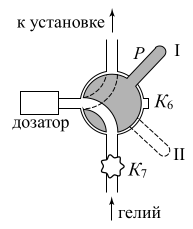
\includegraphics[width=0.2\textwidth]{3.png} % график для P=40.9 торр
		\caption*{Приложение 3. кран с дозатором}
	\end{figure}
	\begin{figure}[h]
		\centering
		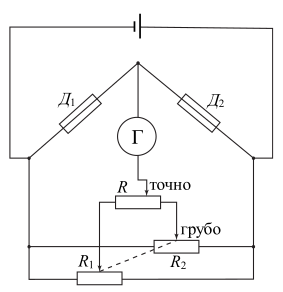
\includegraphics[width=0.2\textwidth]{4.png} % график для P=40.9 торр
		\caption*{Приложение 4. мостовая электрическая схема}
	\end{figure}
	\begin{figure}[h]
		\centering
		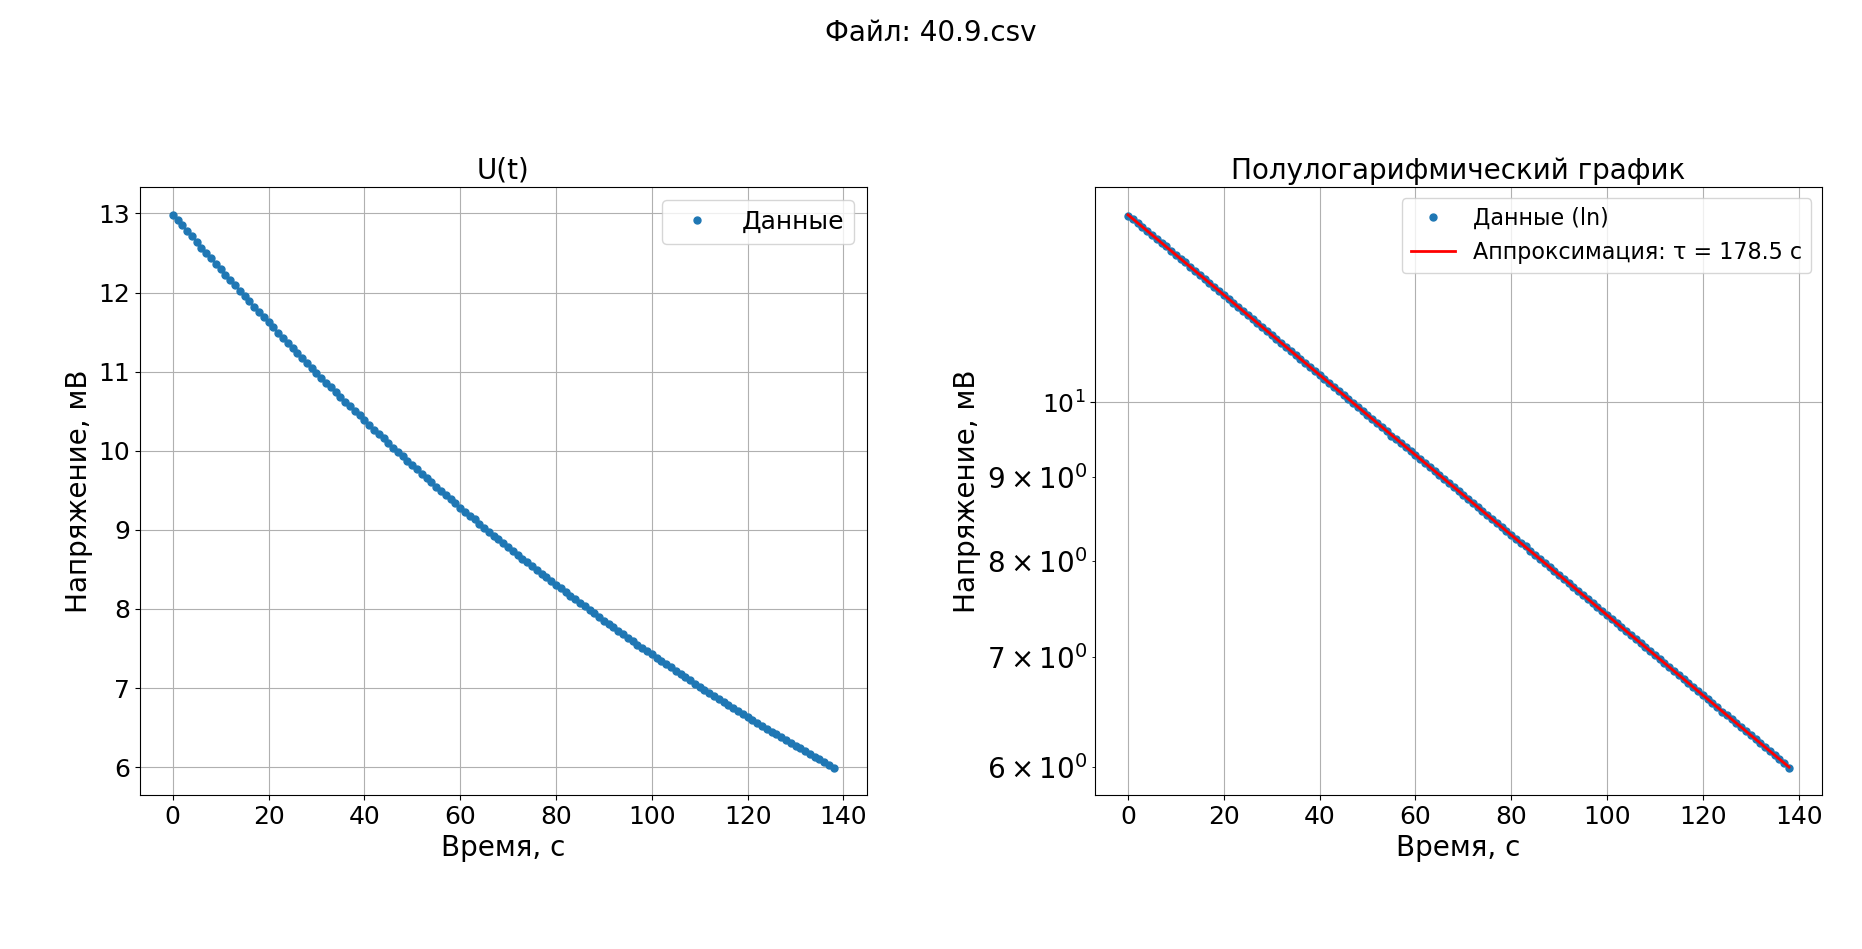
\includegraphics[width=0.8\textwidth]{40.png} % график для P=40.9 торр
		\caption*{Приложение 5. Зависимость \(U(t)\) и её аппроксимация для \(P = 40.9\) торр}
	\end{figure}
	
	\begin{figure}[h]
		\centering
		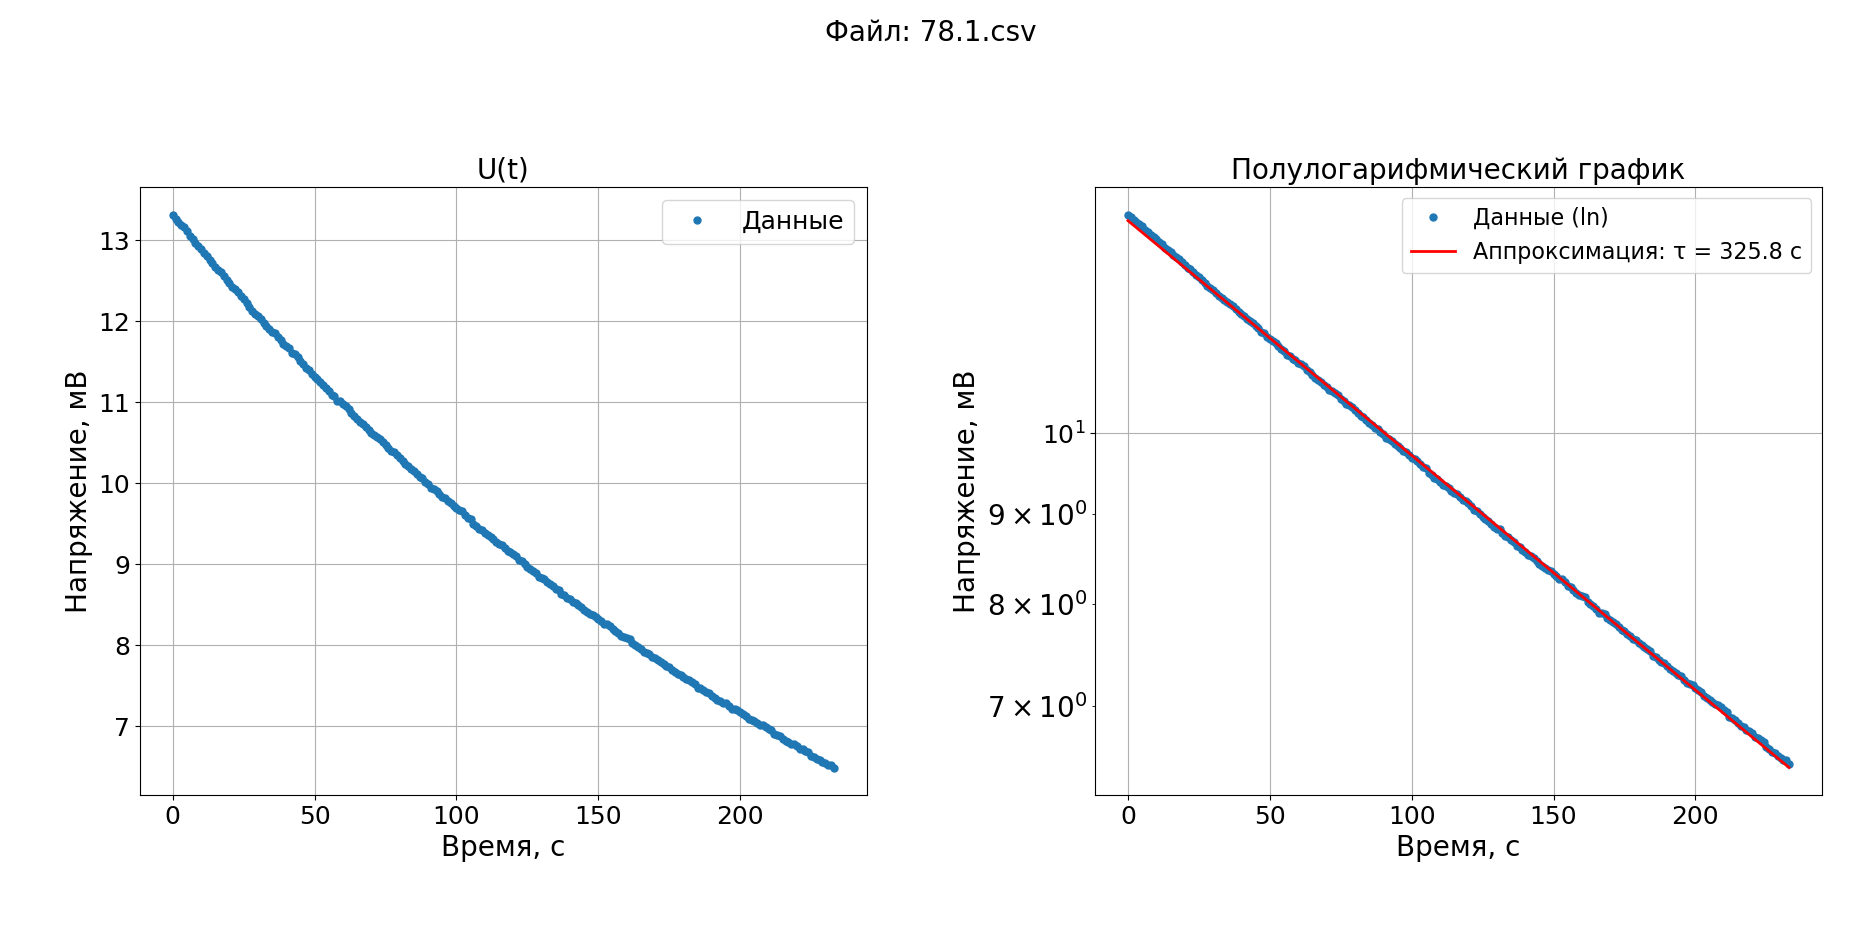
\includegraphics[width=0.8\textwidth]{78.png}
		\caption*{Приложение 6. Зависимость \(U(t)\) и её аппроксимация для \(P = 78.1\) торр}
	\end{figure}
	
	\begin{figure}[h]
		\centering
		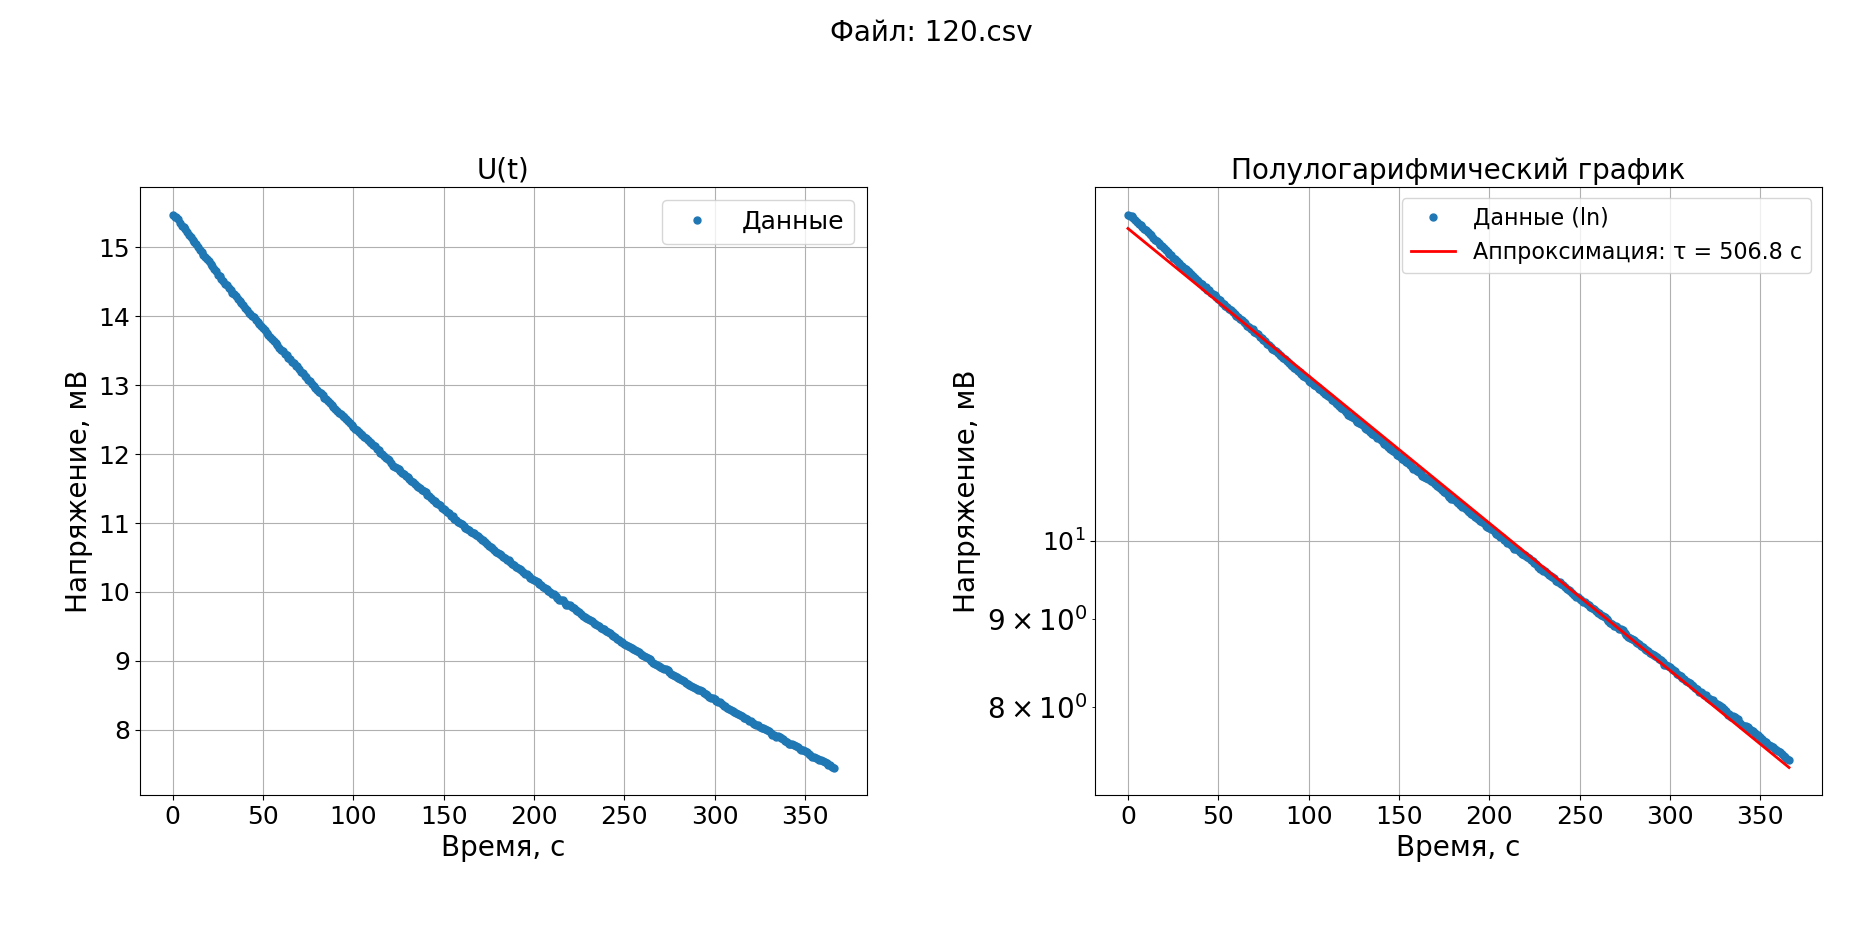
\includegraphics[width=0.8\textwidth]{120.png}
		\caption*{Приложение 7. Зависимость \(U(t)\) и её аппроксимация для \(P = 120\) торр}
	\end{figure}
	
	\begin{figure}[h]
		\centering
		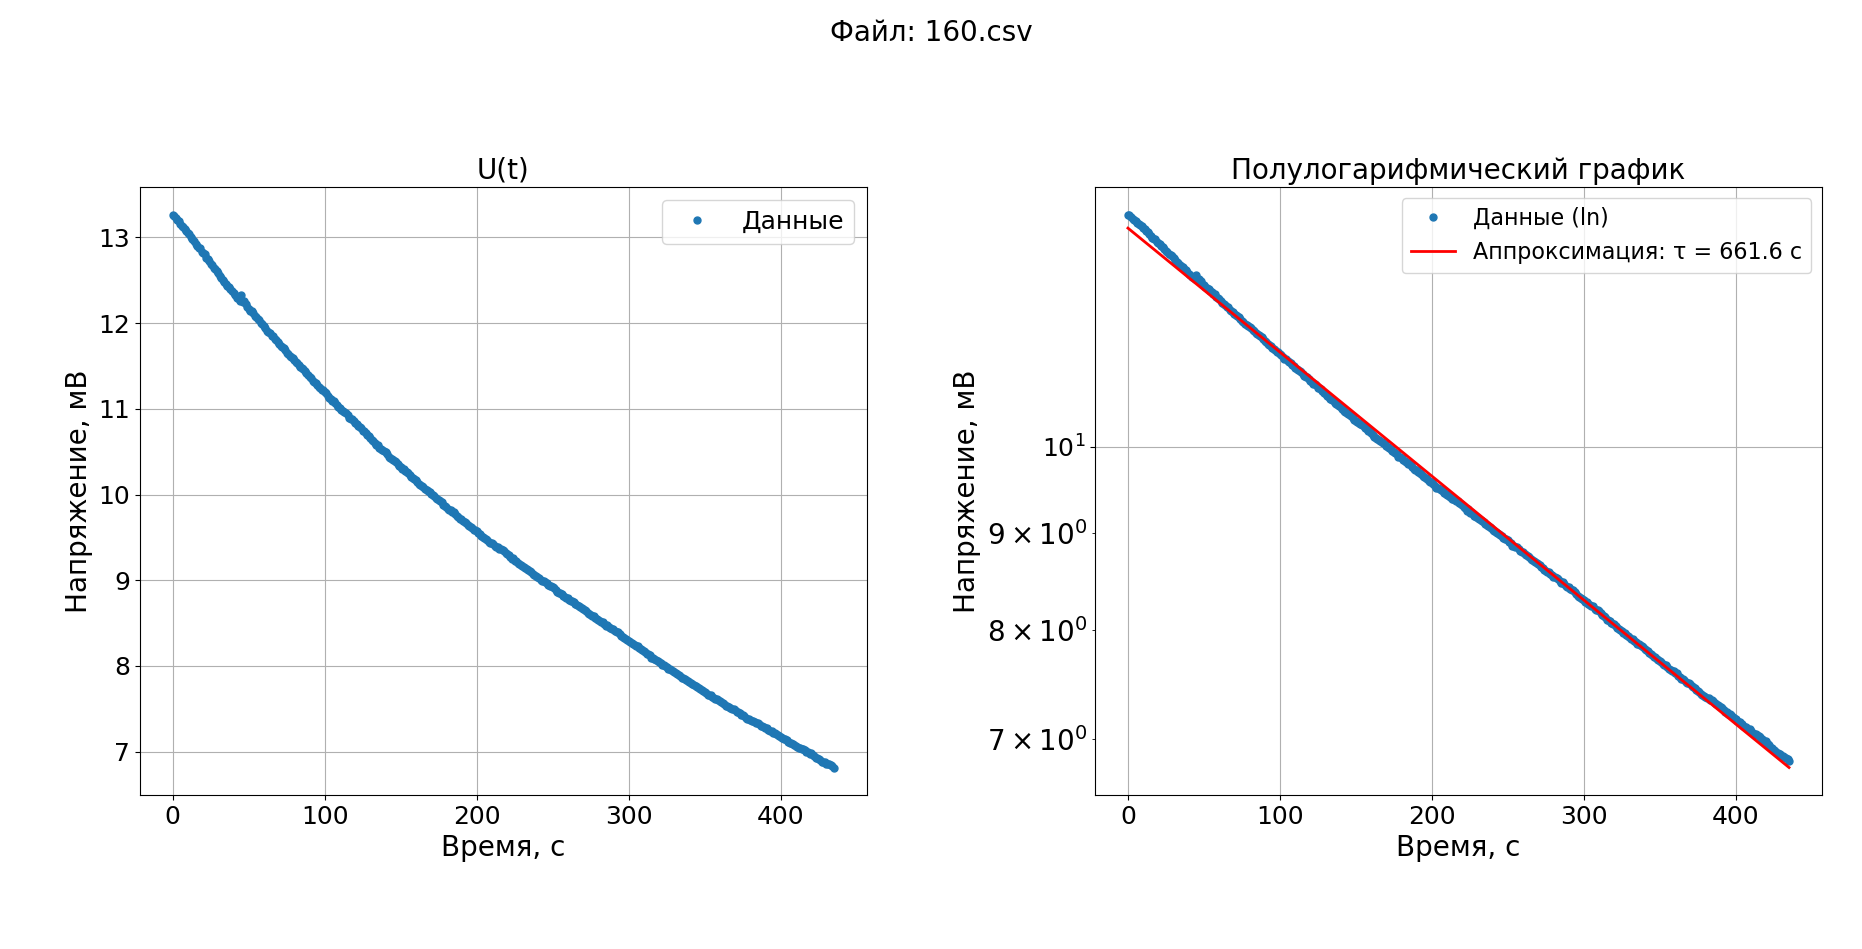
\includegraphics[width=0.8\textwidth]{160.png}
		\caption*{Приложение 8. Зависимость \(U(t)\) и её аппроксимация для \(P = 160\) торр}
	\end{figure}
	
	\begin{figure}[h]
		\centering
		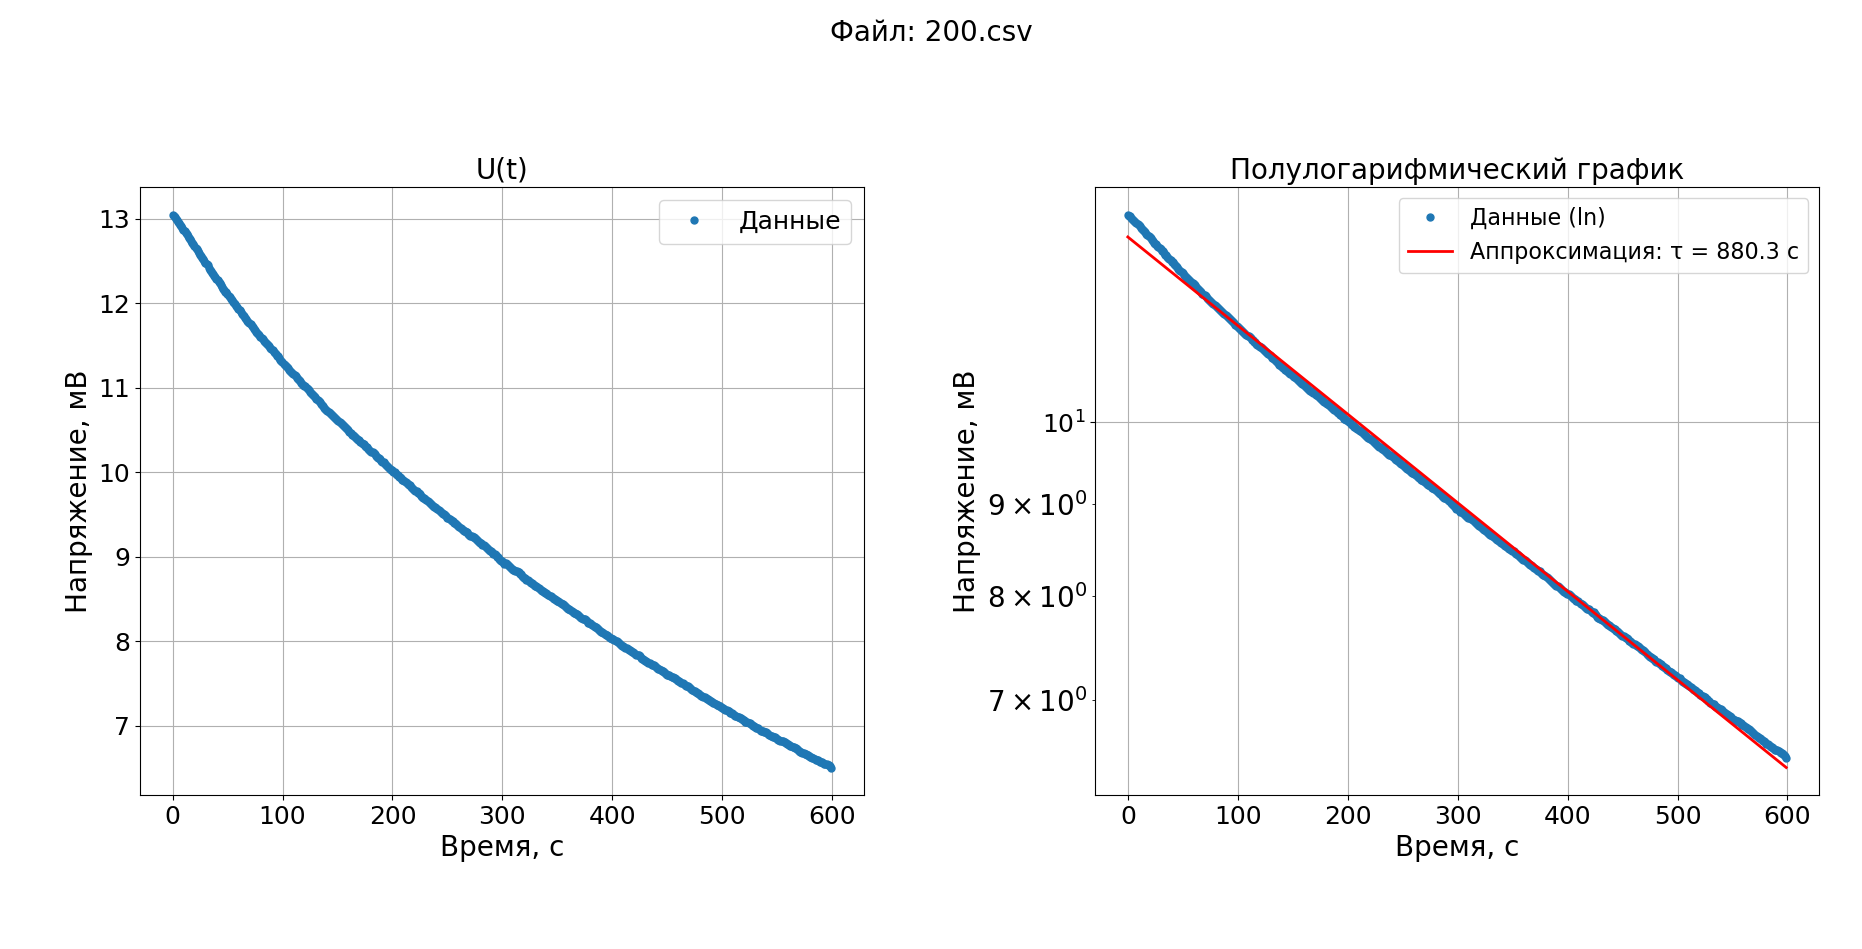
\includegraphics[width=0.8\textwidth]{200.png}
		\caption*{Приложение 9. Зависимость \(U(t)\) и её аппроксимация для \(P = 200\) торр}
	\end{figure}
	
	\begin{figure}[h]
		\centering
		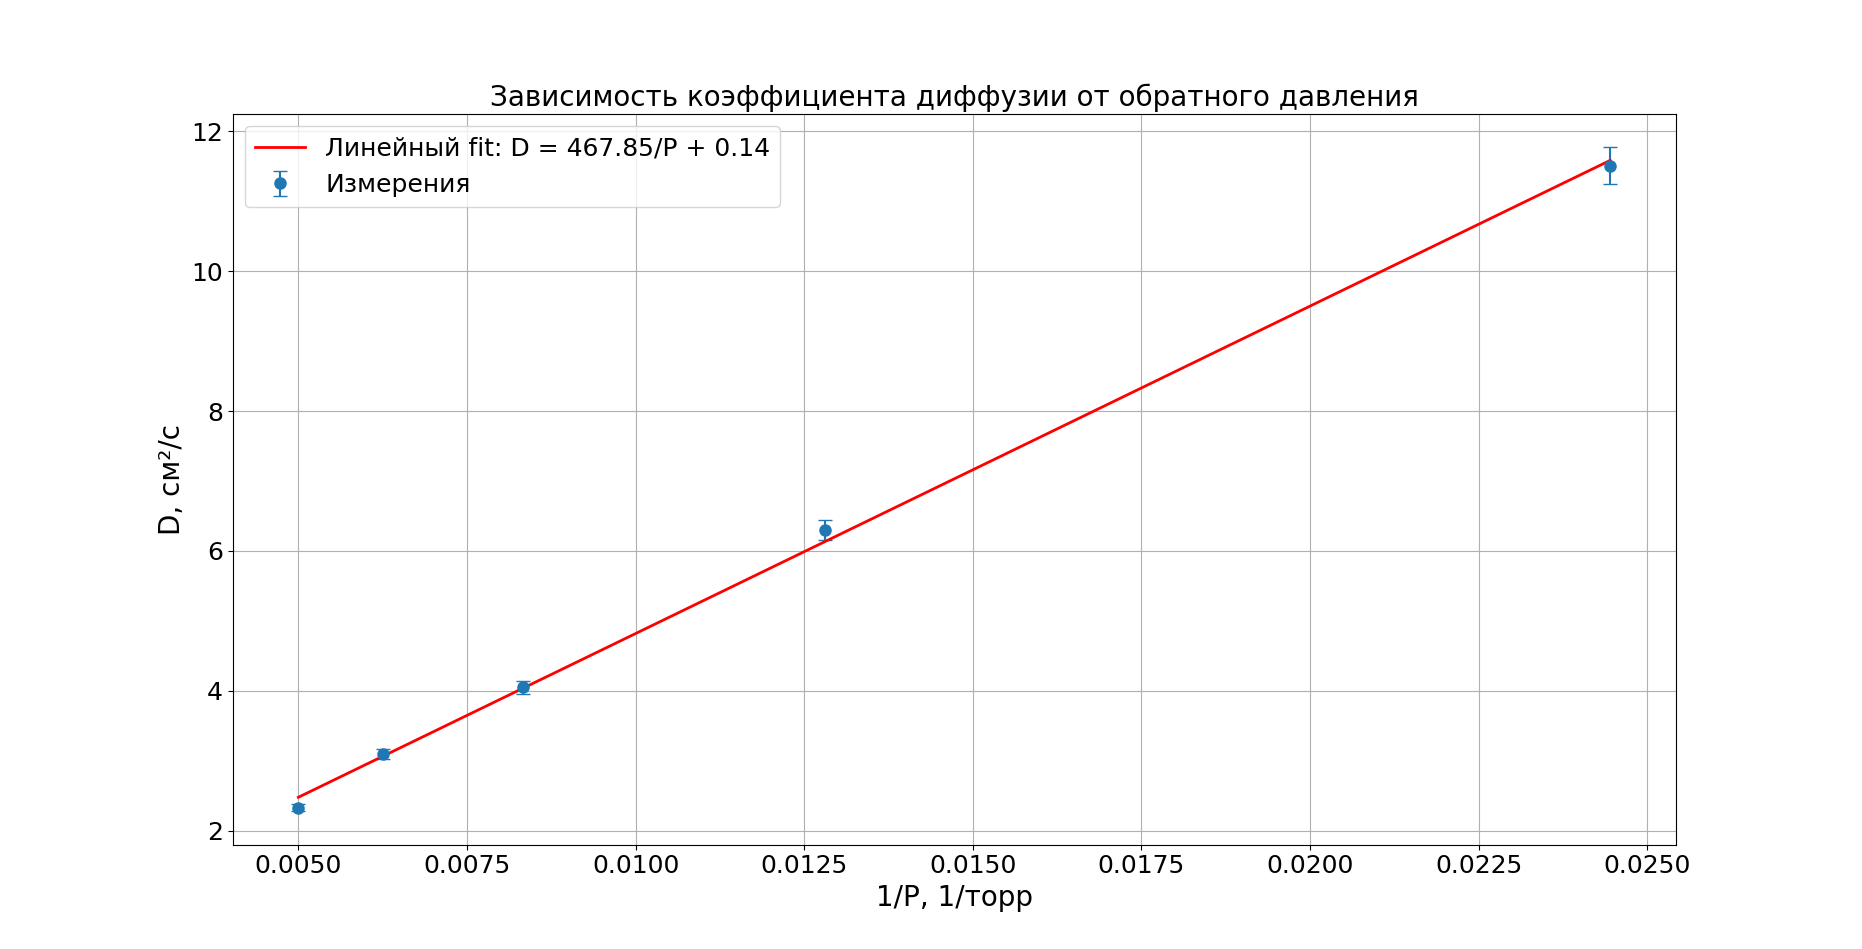
\includegraphics[width=0.9\textwidth]{D.png}
		\caption*{Приложение 10. График зависимости \(D\) от \(1/P\) с линейной аппроксимацией}
	\end{figure}

\end{document}